\documentclass[../MATLAB_Primer.tex]{subfiles}
\begin{document}
An array is a collection of elements of the same data type whose contents can be accessed via indexing. Arrays are fundamental data structures in all coding languages and thus it is important to quickly become familiar with them.  1D arrays are referred to as vectors and can be formatted as row vectors (horizontal) or column vectors (vertical). 2D arrays are referred to as matrices.\\

In mathematics the concept of a vector or a matrix is readily captured through the array. MATLAB is a programming language geared towards numeric computing, and as such offers significant functionality in terms of array operations. MATLAB itself is an abbreviation of the words 'Matrix Laboratory'.

\subsection{Array Declaration}
To create an array you can follow the convention outlined in the examples below.  Row elements (typically of type $\texttt{int}$ or $\texttt{double}$) are separated by either a comma or a space and new rows are defined using a semicolon.\\

Example 1:\\

\textit{input:}
\begin{lstlisting}
row = [1 2 3 4]
% could equally write: row = [1,2,3,4]
\end{lstlisting}
\textit{output:}
\begin{center}
    row = 
$\begin{bmatrix}
 1 & 2 & 3 & 4
\end{bmatrix}$
\end{center}

Example 2:\\

\textit{input:}
\begin{lstlisting}
col = [1;2;3;4]
\end{lstlisting}
\textit{output:}
\begin{center}
col = 
$\begin{bmatrix}
 1\\
 2\\
 3\\
 4
\end{bmatrix}$
\end{center}

Example 3:\\

\textit{input:}
\begin{lstlisting}
matrix = [1, 2, 3, 4; 
          5, 6, 7, 8; 
          9, 10, 11, 12;
          13, 14, 15, 16]
% in one line: matrix = [1,2,3,4; 5,6,7,8; 9,10,11,12; 13,14,15,16]
\end{lstlisting}
\textit{output:}
\begin{center}
matrix = 
$\begin{bmatrix}
 1 & 2 & 3 & 4\\ 
 5 & 6 & 7 & 8\\
 9 & 10 & 11 & 12\\
 13 & 14 & 15 & 16
\end{bmatrix}$
\end{center}

MATLAB offers useful functions to create commonly needed matrices. A list of these functions relevant to the project scope can be found below.
\begin{table}[H]
\caption{Built-in matrix template functions with links to documentation}
    \begin{center}
        \begin{tabular}{| C{2.5cm} | m{12cm}|}
            \hline
            \textbf{MATLAB Syntax} & \textbf{Description}\\
            \hline 
            \href[pdfnewwindow=true]{https://www.mathworks.com/help/matlab/ref/linspace.html}{\color{blue}linspace(x1,x2,n)} & Returns an array of $n$ evenly spaced points between $x1$ and $x2$\\
            \hline
            \href{https://www.mathworks.com/help/matlab/ref/zeros.html}{\color{blue}zeros(sz)} & Returns a matrix of size $sz$ with zeros in every location\\
            \hline
            \href{https://www.mathworks.com/help/matlab/ref/ones.html}{\color{blue}ones(sz)} & Returns a matrix of size $sz$ with ones in every location\\
            \hline
            \href{https://www.mathworks.com/help/matlab/ref/eye.html}{\color{blue}eye(n)} & Returns the $n\times n$ identity matrix\\
            \hline
            \href{https://www.mathworks.com/help/matlab/ref/diag.html}{\color{blue}diag(v)} & Returns a diagonal matrix from a vector $v$ or returns the diagonal entries of a matrix as a vector\\
            \hline
        \end{tabular}
        \label{tab:matrix definitions}
    \end{center}
\end{table}

Example 4:\\

\textit{input:}
\begin{lstlisting}
x = linspace(0,2*pi,100); % 100 evenly spaced points between 0 and 2pi
y = sin(x);

plot(x,y);
% linspace is extremely useful in evaluating functions 
\end{lstlisting}
\textit{output:}
\begin{figure}[H]
    \centering
    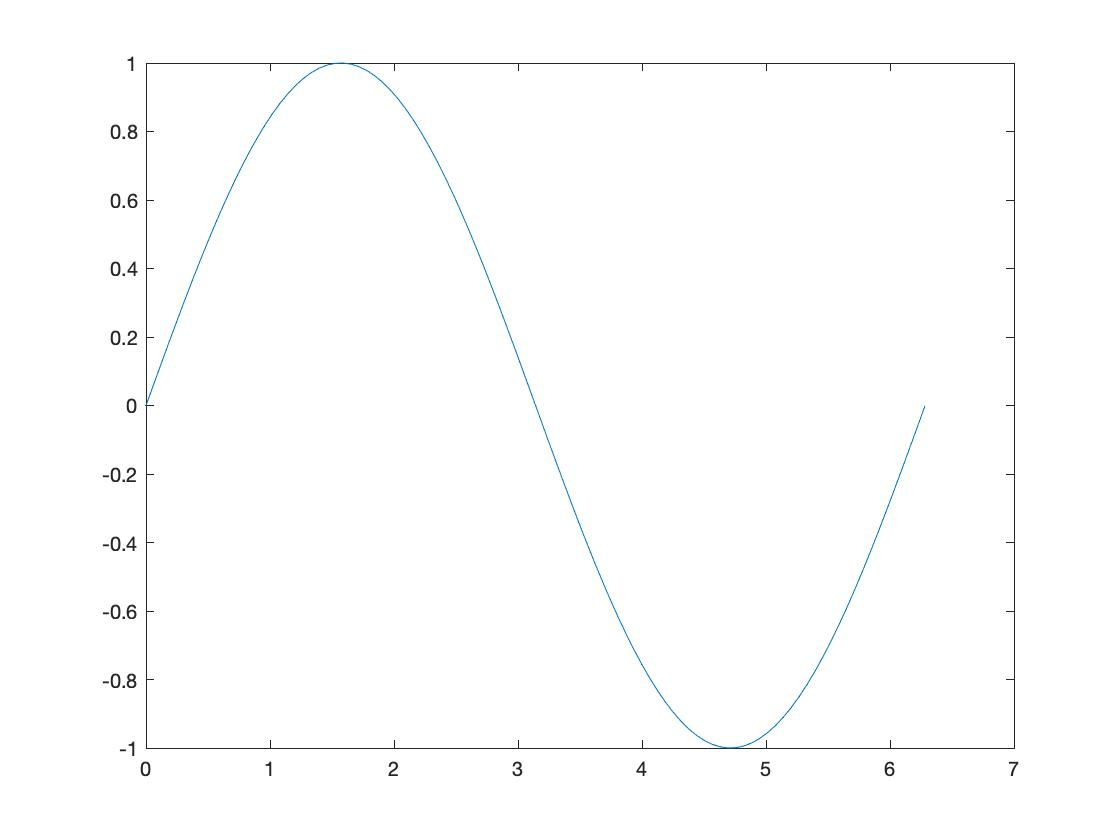
\includegraphics[width=350pt]{images/sample_plot.jpg}
    \caption{Using linspace to efficiently plot sin(x) on [0,2$\pi$]}
    \label{fig:sample_plot}
\end{figure}

Example 5:\\

\textit{input:}
\begin{lstlisting}
% generating the 3x3 identity matrix using different methods 

% manually 
I = [1,0,0; 0,1,0; 0,0,1];

% eye
I = eye(3);

% diag 
v = ones(1,3); % 1x3 row vector [1 1 1]
I = diag(v);

\end{lstlisting}

Oftentimes matrix functions can be called with different parameters than the default examples above.  Refer to the resources linked in the table above for further information.

\subsection{Array Indexing} \label{Indexing}

Indexing in MATLAB is 1-based (first element indexed by a 1 instead of 0) and elements are accessed using parentheses.  For multi-dimensional arrays, either 2 indices $(i,j)$ specifying the $(row,col)$ location, or a single index counting column-wise can be used.\\

Example 1:\\

\textit{input:}
\begin{lstlisting}
A = [1,2;
     3,4];

v = [3, 2, 1];

result = A(1,1) + v(3) % result = 1 + 1
\end{lstlisting}

\textit{output:}
\begin{center}
    result = 2
\end{center}

Additionally, you can use the keyword $end$ to specify the index of the last element in a row or column.  $end$ can be used arithmetically in indexing (e.g. ``$end$-1" is the second last index).\\

Example 2:\\

\textit{input:}
\begin{lstlisting}
A = [1, 2, 3;
     4, 5, 6;
     7, 8, 9]
     
result = A(end, 1) + A(2, end-1) % result = 7 + 5
\end{lstlisting}

\textit{output:}
\begin{center}
    result = 12
\end{center}

\subsection{Array Operations} \label{Basic}
Matrix addition and subtraction is performed element-wise as you'd expect and can be executed simply by using the + and - operators. Array  multiplication or power operations; however, can be performed element-wise \textbf{or} with matrix multiplication. To perform element-wise operations, you are required to use the '.' prefix. Consider the following example:\\

Example 1:\\

\textit{input:}
\begin{lstlisting}
A = [1,0; 
     0,2];
     
B = [0,5; 
     3,0];

C = A + B; % addition is done element-wise

% 2x2 identity matrix
I = eye(2);

result1 = I*C % matrix multiplication
result2 = I.*C % element-wise multiplication
result3 = 3.*(C.^2)
\end{lstlisting}
\textit{output:}

\begin{center}
    result1 = 
    $\begin{bmatrix}
     1 & 0\\
     0 & 1
    \end{bmatrix}
    \begin{bmatrix}
     1 & 5\\
     3 & 2
    \end{bmatrix} = 
    \begin{bmatrix}
     1 & 5\\
     3 & 2
    \end{bmatrix}$\\
\end{center}

\begin{center}
    result2 = 
    $\begin{bmatrix}
     1*1 & 0*5\\
     0*3 & 1*2
    \end{bmatrix} = 
    \begin{bmatrix}
     1 & 0\\
     0 & 2
    \end{bmatrix}$
\end{center}

\begin{center}
    result3 =
    $\begin{bmatrix}
     3*(1)^{2} & 3*(5)^{2}\\
     3*(3)^{2} & 3*(2)^{2}
    \end{bmatrix} = 
    \begin{bmatrix}
     3 & 75\\
     27 & 12
    \end{bmatrix}$
\end{center}

\subsubsection{Built-in Array Functions}
It is very common for there to already exist a function within MATLAB that can perform a standard matrix operation. In the table below several such functions are provided with links to the official documentation. 

\begin{table}[H]
\caption{General Matrix/Array Commands}
    \begin{center}
        \begin{tabular}{| C{3cm} | m{12cm}|}
            \hline
            \textbf{MATLAB Syntax} & \textbf{Description}\\
            
            \hline
            \href{https://www.mathworks.com/help/matlab/ref/size.html}{\color{blue}size(arr)} & Returns a row vector containing the dimensions of an array, $arr$\\
            \hline
            
            \href{https://www.mathworks.com/help/matlab/ref/sum.html}{\color{blue}sum(arr)} & Returns the sum of array elements along a specified axis.  For matrices the default function call returns a row vector with the sum over columns. \\
            \hline
            
            \href{https://www.mathworks.com/help/matlab/ref/max.html}{\color{blue}max(arr)} & Returns the max values in array $arr$ or matrix along a specific axis (i.e. row or column)\\
            \hline
            
            \href{https://www.mathworks.com/help/matlab/ref/min.html}{\color{blue}min(arr)} & Returns the min values in array $arr$ or matrix along a specific axis (i.e. row or column). \\
            \hline
            
            \href{https://www.mathworks.com/help/matlab/ref/sort.html}{\color{blue}sort(arr)} & Returns a sorted structure given an array, $arr$, in ascending order by default.  This direction can be modified by changing function parameters.\\
            
            \hline
            \href{https://www.mathworks.com/help/matlab/ref/arrayfun.html}{\color{blue}arrayfun(f, arr)} & Applies function, $f$, to each element in the array $arr$.  $f$ must be a \href{https://www.mathworks.com/help/matlab/matlab_prog/creating-a-function-handle.html}{\color{blue}function handle}\\
            \hline
        \end{tabular}
        \label{tab:array_functions}
    \end{center}
\end{table}

Example 1:\\

\textit{input:}
\begin{lstlisting}
A = [5,6;
     3,8]

v = [1,2,3,4,5]; 

disp(size(A))   % dim(A) = 2x2
disp(size(v))   % dim(v) = 1x5
\end{lstlisting}
\textit{output:}

\begin{center}
    size(A) = [2\quad2],\quad size(v) = [1\quad5]
\end{center}

Example 2:\\

\textit{input:}
\begin{lstlisting}
A = [5,6;
     3,8]

max_cols = max(A,[],1) % returns the max value of each column
max_rows = max(A,[],2) % returns the max value of each row 


sum_cols = sum(A,1) % returns the sum of each column
sum_rows = sum(A,2) % returns the sum of each row 


\end{lstlisting}
\textit{output:}

\begin{center}
    max\_cols =
    $\begin{bmatrix}
     5 & 8\\
    \end{bmatrix}$,\quad
   max\_rows =
    $\begin{bmatrix}
     6\\8
    \end{bmatrix}$,\quad
    sum\_cols =
    $\begin{bmatrix}
     8 & 14\\
    \end{bmatrix}$,\quad
    sum\_rows =
    $\begin{bmatrix}
     11 \\ 11
    \end{bmatrix}$
\end{center}

Example 3:\\

\textit{input:}
\begin{lstlisting}
% let d be the distances from some agents to a reference point
% sort according to closest then farthest from the reference point

d = [1, 3.3, 0.5, 0.1, 1.2, 2, 6];  % unordered collection

near = sort(d, 'ascend')
far = sort(d, 'descend')

\end{lstlisting}
\textit{output:}

\begin{center}
    near = $\begin{bmatrix}
     0.1 & 0.5 & 1 & 1.2 & 2 & 3.3 & 6
    \end{bmatrix}$,\quad
    far = $\begin{bmatrix}
     6 & 3.3 & 2 & 1.2 & 1 & 0.5 & 0.1
    \end{bmatrix}$
\end{center}
%need this for the spacing ://
\begin{center}
     
\end{center}
In addition to general utility functions for arrays, MATLAB also offers convenient functions for common linear algebra operations. 

\begin{table}[H]
    \caption{Useful Functions for Linear Algebra}
    \begin{center}
        \begin{tabular}{| C{3cm} | m{12cm} |}
                \hline
                \textbf{MATLAB Syntax} & \textbf{Description}\\
            
                \hline
                \href{https://www.mathworks.com/help/matlab/ref/det.html}{\color{blue}det(A)} & Returns the determinant of a square matrix $A$\\
                \hline
                
                \href{https://www.mathworks.com/help/matlab/ref/eig.html}{\color{blue}eig(A)} & Returns a column vector containing the eigenvalues of a square matrix $A$\\
                \hline
                
                \href{https://www.mathworks.com/help/matlab/ref/inv.html}{\color{blue}inv(A)} & Returns the inverse of a square matrix $A$\\
                \hline
                
                \href{https://www.mathworks.com/help/matlab/ref/transpose.html}{\color{blue}transpose(A)} or A' & Returns the transpose of a matrix $A$\\
                \hline
                
                \href{https://www.mathworks.com/help/matlab/ref/cross.html}{\color{blue}cross(u,v)} & Returns the cross products given two arrays $u$ and $v$\\
                \hline
                
                \href{https://www.mathworks.com/help/matlab/ref/dot.html}{\color{blue}dot(u,v)} & Returns the dot product given two arrays $u$ and $v$\\
                \hline
        \end{tabular}
    \end{center}
    \label{tab:linalg_functions}
\end{table}

Example 4:\\

\textit{input:}
\begin{lstlisting}
% create some basis/column vectors 
i = [2;0;0];
j = [0;0.5;0];
k = cross(i,j);

A = [i j k] % 3x3 matrix with column vectors i,j,k

% find determinant of A
det_A = det(A)

% find the max and min eigenvalues for A 
eig_vals = eig(A); % {2,0.5,1}
max_eig = max(eig_vals) % 2
min_eig = min(eig_vals) % 0.5
\end{lstlisting}
\textit{output:}\\

\begin{center}
    det$\_$A = 1,\quad
    max$\_$eig = 2,\quad
    min$\_$eig = 0.5
\end{center}

Example 5:\\

\textit{input:}
\begin{lstlisting}
% some methods for the dot product of u and v
u = [1,2,3];
v = [4,5,6];

% manual
result = u*v'; % equivalent to u*transpose(v)

result = sum(u.*v); 

% built-in
result = dot(u,v)
\end{lstlisting}
\textit{output:}\\

\begin{center}
    result = 32
\end{center}

Whenever possible, use a pre-written function provided by MATLAB instead of writing them on your own. 


\subsection{Size \& Dimension Manipulation} 
We often need to manipulate the dimension of an array to store new information (an increase in dimensionality) or to make our data structure compatible with a pre-existing function.  The term used to describe the ``splicing" of two separate arrays is called \textbf{concatenation}. We can also change the shape of an array while still keeping all the information through \textbf{reshaping}.

\subsubsection{Concatenation}
Suppose we have the two matrices:
\[
A = 
\begin{bmatrix}
1 & 2 & 3\\
4 & 5 & 6\\
7 & 8 & 9\\
\end{bmatrix}
\text{    and    }
B = 
\begin{bmatrix}
1 & 1 & 1\\
1 & 1 & 1\\
\end{bmatrix}
\]
And we want to attach B onto A. We can only do this in one way is by adding B to the bottom of A as rows 4 and 5. This would look like:
\[
\text{concatenation(A,B)} = 
\begin{bmatrix}
1 & 2 & 3\\
4 & 5 & 6\\
7 & 8 & 9\\
1 & 1 & 1\\
1 & 1 & 1\\
\end{bmatrix}
\]
We can not add B to A as columns since the number of rows of A and B differ. This will also prevent B from being added to A in the third dimension.\\

In MATLAB we can make use of the following two functions for concatenation:

\begin{table}[H]
\caption{MATLAB Functions for Array Concatenation}
    \begin{center}
        \begin{tabular}{| C{3cm} | m{12cm}|}
            \hline
            \textbf{MATLAB Syntax} & \textbf{Description}\\
            
            \hline
            \href{https://www.mathworks.com/help/matlab/ref/horzcat.html}{\color{blue}horzcat(A,B)} & Concatenates matrices $A$ and $B$ along the horizontal axis\\
            \hline
            
            \href{https://www.mathworks.com/help/matlab/ref/vertcat.html}{\color{blue}vertcat(A,B)} & Concatenates matrices $A$ and $B$ along the vertical axis\\
            \hline
        \end{tabular}
        \label{tab:more_array_functions}
    \end{center}
\end{table}

Example 1: \\

\textit{input:}
\begin{lstlisting}
% size(A) = (4,2)
A = [1,2;
     3,4;
     5,6;
     7,8];  

% size(B) = (2,2)
B = [9,10;
     11,12];       

vertcat(A,B)
\end{lstlisting}
\textit{output:}
\begin{center}
    ans = $\begin{bmatrix}
     1 & 2\\
     3 & 4\\
     5 & 6\\
     7 & 8\\
     9 & 10\\
     11 & 12\\
    \end{bmatrix}$
\end{center}

Example 2:\\

\textit{input:}
\begin{lstlisting}
A = [1 2 3 4 5];    % size(A) = (1,5)
B = [6;7;8;9;10];   % size(B) = (5,1)

horzcat(A,transpose(B))
\end{lstlisting}
\textit{output:}
\begin{center}
    ans = $\begin{bmatrix}
     1 & 2 & 3 & 4 & 5 & 6 & 7 & 8 & 9 & 10\\
    \end{bmatrix}$
\end{center}

\subsubsection{Reshaping}
Reshaping involves manipulating the dimensions of a data structure for the purpose of representing information in a different manner.  This is often done so that we can pass our array to a function that requires input arguments of a specific shape. The importance of this idea extends beyond simply MATLAB to the many other coding languages as well. 

\begin{table}[H]
\caption{MATLAB Functions for Array Manipulation}
    \begin{center}
        \begin{tabular}{| C{3cm} | m{12cm}|}
            \hline
            \textbf{MATLAB Syntax} & \textbf{Description}\\
            
            \hline
            \href{https://www.mathworks.com/help/matlab/ref/reshape.html}{\color{blue}reshape(A, sz)} & Reshapes array $A$ into an array of size $sz$\\
            \hline
            
        \end{tabular}
        \label{tab:array_manipulation}
    \end{center}
\end{table}

Example 1:\\

\textit{input:}
\begin{lstlisting}
A = [1,2;
     3,4;
     5,6]
     
A_reshaped = reshape(A, [2,3])
% we've reshaped a 3x2 array to a 2x3 one
\end{lstlisting}
\textit{output:}
\begin{center}
    A = $\begin{bmatrix}
     1 & 2\\
     3 & 4\\
     5 & 6\\
    \end{bmatrix}$,\quad
    A\_reshaped = $\begin{bmatrix}
     1 & 3 & 5\\
     2 & 4 & 6\\
    \end{bmatrix}$
\end{center}

Example 2:\\

\textit{input:}
\begin{lstlisting}
% many machine learning models take in nx1 feature vectors as inputs 
% we can 'flatten' high dimensional information into a 1D vector with reshape

agent_coords = [0,0,0; 1,1,1; 5,2,1]

feature_vector = reshape(agent_coords, [9,1])
% note: 3x3 array has 9 elements...
\end{lstlisting}
\textit{output:}
\begin{center}
    agent\_coords = $\begin{bmatrix}
     0 & 0 & 0\\
     1 & 1 & 1\\
     5 & 2 & 1\\
    \end{bmatrix}$,\quad
    feature\_vector = $\begin{bmatrix}
     0\\1\\5\\0\\1\\2\\0\\1\\1\\
    \end{bmatrix}$
\end{center}

\subsection{Array Logic}
Since arrays efficiently store information via elements, it is often useful to know which elements satisfy certain conditions. Similar to scalar-valued expressions, we can construct logical statement using arrays in a very intuitive manner.\\

When we evaluate a logical expression using arrays, the output is also an array with the same dimension as the original with 1's assigned to elements which satisfy the prescribed relation, and 0's for those that don't.  Observe the examples below to see how powerful this can be.\\ 

Example 1:\\

\textit{input:}
\begin{lstlisting}
a = [1,2,3,4,5,6,7,8];

a>=4
\end{lstlisting}
\textit{output:}
\begin{center}
    ans = 
    $\begin{bmatrix}
    0 & 0 & 0 & 1 & 1 & 1 & 1 & 1\\
    \end{bmatrix}$
\end{center}

Example 2:\\

\textit{input:}
\begin{lstlisting}
% suppose D contains the relative distances from some agents to one another 
% where D(i,j) = D(j,i) = distance(agent_i, agent_j) 
D = [0,1,5; 
     1,0,2; 
     5,2,0];

% find which agents are less than 2 units apart
D_bool = D<2

% recover indices of elements satisfying condition above
find(D_bool)
\end{lstlisting}
\textit{output:}
\begin{center}
    D\_bool = 
    $\begin{bmatrix}
    1 & 1 & 0\\
    1 & 1 & 0\\
    0 & 0 & 1\\
    \end{bmatrix}$,\quad 
    ans = 
    $\begin{bmatrix}
    1\\2\\4\\5\\9\\
    \end{bmatrix}$
\end{center}
Recall that 2D arrays can be indexed by a single integer which counts column-wise in a manner referred to as \href{https://www.mathworks.com/help/matlab/math/array-indexing.html#MatrixIndexingExample-2}{\color{blue}linear indexing}.\\

Example 3:\\

\textit{input:}
\begin{lstlisting}
%random pairwise distances between agents 
distances = [1,2,3; 
             4,5,6; 
             7,8,9];

%agent radii of communication
rc = [2;
      6;
      7];

distances<=rc
\end{lstlisting}
\textit{output:}
\begin{center}
    ans = 
    $\begin{bmatrix}
    1 & 1 & 0\\
    1 & 1 & 1\\
    1 & 0 & 0
    \end{bmatrix}$
\end{center}

%need another space
\begin{center}
     
\end{center}

In the example above we're essentially asking the 3 following questions:
\begin{itemize}
    \item which pairwise distances in row vector [1,2,3] are less than or equal to a communication radius of 2?
    \item which pairwise distances in row vector [4,5,6] are less than or equal to a communication radius of 6?
    \item which pairwise distances in row vector [7,8,9] are less than or equal to a communication radius of 7?
\end{itemize}

\begin{center}
     
\end{center}

We can also make use of an idea known as \textbf{logical indexing} where we pass the output of a logical expression as an index to our data structure to access the elements which satisfy our predefined conditions.\\ 

Example 4:\\

\textit{input:}
\begin{lstlisting}
%double the odd entries in matrix A 
A = [1,2;3,4];
    
idx = (mod(A,2)==1)    % array with 1's where A is odd

A(idx) = 2*A(idx)   % access odd elements and double
\end{lstlisting}
\textit{output:}
\begin{center}
    idx = 
    $\begin{bmatrix}
    1 & 0\\
    1 & 0\\
    \end{bmatrix}$,\quad
    A =
    $\begin{bmatrix}
    2 & 2\\
    6 & 4\\
    \end{bmatrix}$
\end{center}

\subsection{Cell Arrays}
Cell arrays are a similar to traditional arrays but differ in that they can contain multiple different data types and objects.  In this sense the cell array is a more abstracted version of an array. Cell arrays are useful for grouping related information which is not restricted solely to numeric types.

\subsubsection{Declaration}
The example below runs through the basics of cell array declaration and element accessing/modification. Note that we use curly braces when we define our cell array.\\

Example 1:\\

\textit{input:}
\begin{lstlisting}
% consider a structure representing student grades and overall averages 
grades = {'jack', [50, 83, 90, 92], 79;
          'felix', [85, 90, 94, 73], 86; 
          'nate', [84, 89, 93, 72], 85};
          
% elements accessed using curly braces 
felix_average = grades{2,3}
jack_grades = grades{1,2}
\end{lstlisting}
\textit{output:}
\begin{center}
    felix\_average = 86,\quad
    jack\_grades =
    $\begin{bmatrix}
    50 & 83 & 90 & 92\\
    \end{bmatrix}$
\end{center}

In the example above we created an array-like structure which contains elements of type \texttt{string}, \texttt{int[]}, and \texttt{int}. It helps to think of the cell array as a container where elements are anything you want them to be (even other cells). 

\subsubsection{cellfun}
\texttt{cellfun} is a utility function which allows one to apply a function to each cell in a cell array. The output is structure with the same dimensions of the cell array, where each entry is the function applied to the corresponding entry in the cell array.\\

\begin{table}[H]
\caption{MATLAB Functions for Array Manipulation}
    \begin{center}
        \begin{tabular}{| C{3cm} | m{12cm}|}
            \hline
            \textbf{MATLAB Syntax} & \textbf{Description}\\
            
            \hline
            \href{https://www.mathworks.com/help/matlab/ref/cellfun.html}{\color{blue}cellfun(func, C)} & Applies function $func$ to every cell in cell array $C$.  Here, $f$ must be a \href{https://www.mathworks.com/help/matlab/matlab_prog/creating-a-function-handle.html}{\color{blue}function handle}\\
            \hline
            
        \end{tabular}
        \label{tab:cell_array}
    \end{center}
\end{table}

Example 1:\\

\textit{input:}
\begin{lstlisting}
C = {1, [1,2,3], [1,2;3,8]};    %stores scalar, array, and matrix
f = @(x) max(x,[],'all');       %max across all dimensions

cellfun(f,C)
\end{lstlisting}
\textit{output:}
$$
    ans = 
    \begin{bmatrix}
    1 & 3 & 8
    \end{bmatrix}
$$

Example 2:\\

\textit{input:}
\begin{lstlisting}
C = {1, [1,2,3], [1,2;3,8]};    %stores scalar, array, and matrix
f = @(x) sum(x,2);              %sum over rows 

cellfun(f,C, 'UniformOutput', false)    %outputs don't have to be scalar
\end{lstlisting}
\textit{output:}
$$
    ans = 
    \{[1]\} \quad \{[6]\} \quad 
    \{\begin{bmatrix}
    3\\11
    \end{bmatrix}\}
$$

\end{document}